\documentclass[a4paper,10pt]{article}
\usepackage[utf8]{inputenc}
\usepackage[T1]{fontenc}
\usepackage[english]{babel}
\usepackage{caption}
\usepackage{geometry}
\usepackage{graphicx}
\geometry{
	a4paper,
	top=20mm,
}

\begin{document}
	
\title{Google App Engine - Assignment 1}
\author{Jakub Adam \and Matteo Di Pirro}
\date{November 24, 2017}

\maketitle

\section{Question 1}
To explain why we rely on JPA transaction is worthy to explain our data model depicted in Figure 1. We use a four-level tree with a \texttt{CarRentalCompany} as a root. This object contains explicit references to zero or more \texttt{CarType}s, containing references to \texttt{Car}s belonging to that car type. Also each \texttt{Car} entity contains references to zero or more reservations booked for a concrete car.

\begin{figure}[h]
	\centering
	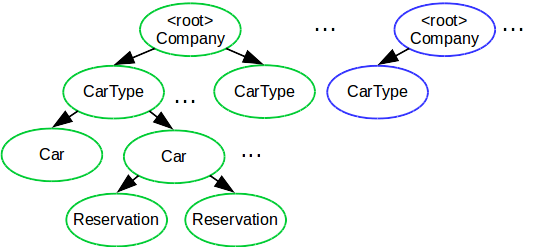
\includegraphics[scale=0.8]{./TreeStructure}
	\caption{Tree structure for data}
\end{figure}

This means that every \texttt{CarRentalCompany} is the root of a different entity group (different colors in picture). Hence, supposing a service with 32 registered car rental companies, the application will have to deal with 32 entity groups. Nonetheless, cross-group transactions operate on a maximum of 25 entity groups. Since they cannot achieve a complete consistency and they come with a higher latency, we prefer JPA transactions. We then decided to solve the confirmation of quotes at the application level. The application confirms all quotes related to a concrete car rental company within one transaction. If any of these transactions fails, the application deletes from the datastore all previous successfully created reservation. As an immediate drawback, it might be possible that we need to set up a lot of transactions (in the worst case 32), but we do not think that is a problem since we do not expect many reservations referring to different car rental companies to be confirmed at the same time.

\section{Question 2}
In such a scenario, user profiles are totally independent on car reservations and they will belong to separate entity groups. Furthermore, a user profile does not have any relationships with other profiles, since information referring to a certain user is completely unrelated to other users. Hence, there is no need for cross-group transactions. Not only they would be useless, but they would slow down the application due to their higher latency. This is the reason why we would apply JPA transactions even in this scenario.

\section{Question 3}
Relying on cross-group transactions only is a drawback for concurrent accesses. When a request tries to confirm quotes, no other request is allowed to operate on the same entity groups for consistency reasons. This is an important limitation in a large-scale cloud application, since the latency will be higher and the responsiveness lower. On the other hand, with JPA transactions, we optimistically believe that everything will be ok, and we manually rollback only if something fails. This comes with the underlying assumption that a **concurrent** confirmation on the same entity group is unlikely. This requires additional time, but, if that assumption is true, the responsiveness will be **normally** higher than with cross-group transactions. 

This can be easily linked with the increasing popularuty on NoSQL databases. One of them is MongoDB, which does not provide consistency guarantees and requires the application to detect wrong situations and to rollback if that is the case. The performance is generally better, even if the application code has to deal explicitly with possible erroneous situations.

\end{document}

